\documentclass{article}
\usepackage{graphicx}
\usepackage{amsmath, amssymb}
\usepackage{hyperref}
%\usepackage{cite}
\usepackage{algorithm}
\usepackage{algorithmic}
\usepackage{caption}
\usepackage{graphicx}
\graphicspath{ {./images/} }
\usepackage{booktabs} % For better table formatting
\usepackage{multirow} % For multirow cells
\usepackage{array} % For custom column alignment
\usepackage{tabularx} % For auto-adjusting table width
\usepackage{booktabs} % For better table formatting
\usepackage{adjustbox} % For scaling the table
\usepackage{geometry} % For better page margins
\usepackage{array}
\usepackage[section]{placeins} % for \FloatBarrier
\PassOptionsToPackage{hyphens}{url}\usepackage{hyperref}

\title{Analyzing Public Sentiment on Controversial Sports Events in YouTube Comments}
\date{}

\begin{document}

\maketitle

\section{Annotation Pipeline and Fine Tuning Details}


\subsection{Algorithm Details and Rationale}
The following outlines the overall pipeline and reasoning behind our stance detection approach:
\begin{itemize}
    \item \textbf{Pipeline Design:} The pipeline starts with data extraction and preprocessing to ensure the quality of the input comments. Given the noisy nature of social media data, thorough cleaning was essential.
    \item \textbf{Model Selection:} For the Underarm Incident, the fine-tuned LLaMA-3.1 (Instruct) family of models were chosen for its ability to process long sequences (up to 2048 tokens) and follow the given instructions (as a few shot prompts) to generate coherent responses, making it suitable for detailed stance detection.
    \item \textbf{Structured Prompts:} We used structured prosmpts to guide the model in classifying comments. This method provided consistent JSON responses, ensuring ease of parsing and reliable extraction of stance labels and reasons.
    \item \textbf{OLLAMA Framework:} For Jonny Bairstow's and Ashwin's events, the OLLAMA framework allowed for scalable and concurrent processing of comments via API calls. This was critical in handling larger datasets and ensuring a rapid turnaround in analysis.
    \item \textbf{Evaluation Metrics:} In addition to the stance labels, we compute evaluation metrics such as accuracy, precision, recall, and F1-score to assess model performance.
\end{itemize}




Figure~\ref{fig:pipeline} presents a flowchart summarizing the stance detection pipeline.




\begin{figure}[ht]
\centering
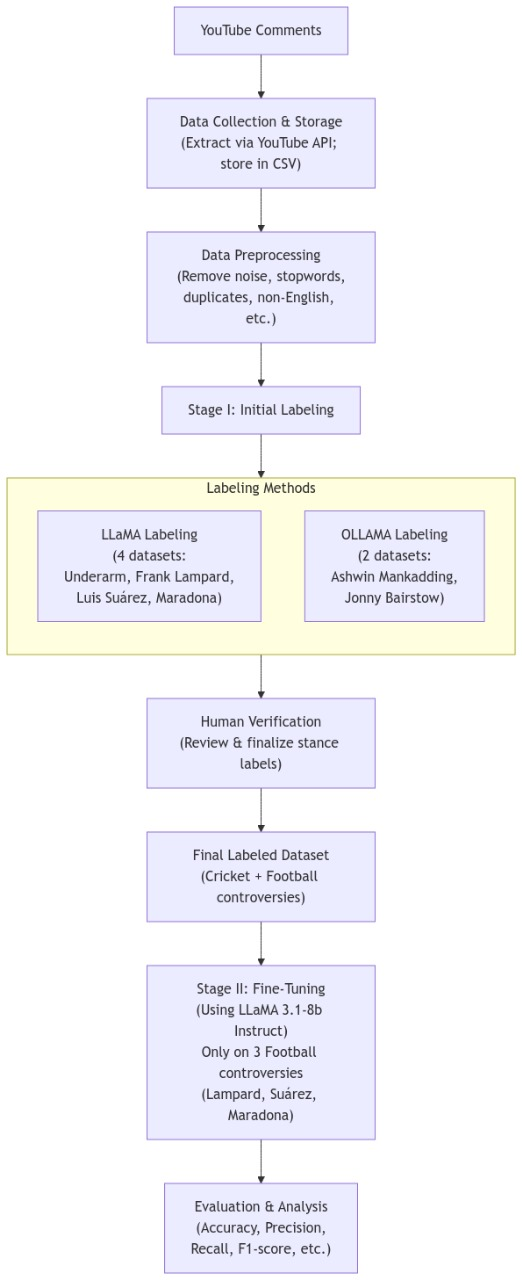
\includegraphics[width=0.48\textwidth]{pipeline.jpg}  % Replace with your actual flowchart image
\caption{Opinion Mining Pipeline Flowchart}
\label{fig:pipeline}
\end{figure}

For clarity, the pseudocode in Algorithm~\ref{alg:pipeline} summarizes the pipeline:

\begin{algorithm}[h]
\caption{Stance Detection Pipeline}
\label{alg:pipeline}
\begin{algorithmic}[1]
\STATE \textbf{Input:} YouTube comments dataset
\STATE \textbf{Preprocessing:} Clean comments by removing noise and duplicated data
\IF{Incident is Underarm}
    \STATE Use the Unsloth LLaMA-3(Instruct) family of models with a structured prompt
    \STATE Parse JSON response to extract stance label and reason
\ELSE
    \STATE Use the OLLAMA framework with API requests and detailed prompts
    \STATE Parse JSON response to extract stance label and reason
\ENDIF
\STATE \textbf{Output:} Stance labels and evaluation metrics (accuracy, precision, recall, F1-score)

\end{algorithmic}
\end{algorithm}
\end{document}